\documentclass[8pt]{mpscheatsheet}
\usepackage{amsmath, amssymb, mathtools, empheq, physics}
\usepackage{xcolor}
\usepackage{graphicx}

\author{Micha Bosshart - bmicha@ethz.ch}
\title{CMEA}

% hide argument given to densify
\newcommand{\densify}[1]{}

\newcommand{\mathbox}[2][]{%
    \begin{center}%
        \boxed{#2} #1
    \end{center}%
}

\begin{document}
    \section{ODE}
        \subsection{Definitions}
    \begin{itemize}
        \item \textbf{Autonomous}: $F(u(t))$ is not an \textit{expl}. func. of time.
        \item \textbf{Non-Autonomous:}  $F(t,u(t))$
        \item \textbf{Linear:} $F(t,u(t)) = A(t) \cdot u(t) + C(t)$, \hfill hom: $C \equiv 0$
        \item \textbf{Non-Linear:} e.g. $u'(t) = \sin(u(t))$
        \item \textbf{Scalar vs. Systems of ODEs}
    \end{itemize}

        \subsubsection{Non-Autonomous \texorpdfstring{$\rightarrow$}{->} Autonomous}
    \vspace{2pt}
    \mathbox{
        u'(t) = F(t,u(t)) \quad \rightarrow \quad w'(t) = G(w(t))
    }
    $$
        w(t) = [u^T(t), \alpha(t)]^T, \quad w(0) = [u^T(0), \alpha(0)]^T
    $$
    $$
        G(w) = w'(t) = [u'(t)^T, \alpha'(t)]^T
    $$
    \vspace{-1em}
        \subsection{Initial Value Problem (IVP)}
    \densify{\vspace{-1em}
    $$
        F\left(t,u,u',\dots,u^{(k)}\right) = 0, \qquad u'(t) = F(t,u(t))
    $$
    $$
        \textrm{with }\ u^{(i)}(0) = u_i, \quad i = 0, \dots, k-1
    $$
    \vspace{-1em}}
    \subsubsection{Lipschitz Theorem}
        If $F(t,u(t))$ is \textbf{lipschitz-continuous}, there exists a time interval $[0,T^*]$, in which the IVP has a \textbf{unique} solution.
        \mathbox{
            \lVert F(t,u) - F(t,u^*) \rVert \leq L \cdot \lVert u - u^* \rVert
        }
        with any vector norm $\lVert \cdot \rVert$ and
        $$
            (u,t), (u^*, t) \in [0,T] \times u, \qquad L >0 
        $$
        \vskip4pt
        \textit{"An lc function is limited in how fast it can change."}

    \section{Numerical Methods}
        \vspace{-1em}\begin{align*}u'(t) &=F(t,u(t))\\u(0) &= u_0\end{align*}
        \subsection{Discretization}
    \vspace{-1em}
    $$
        \textrm{Find }\ \{ u^n \}_{n=0}^N\ \textrm{  s.t. }\ u^n \approx u(t^n) \quad \forall n \in \{ 0,N \}
    $$
    \begin{align*}
        \Delta t &\vcentcolon= \frac{T}{N} & \textrm{time step}\\
        t^n &\vcentcolon= n \cdot \Delta t & \textrm{time level}      
    \end{align*}
    \densify{\subsubsection{Fundamental Thrm of Calculus (FTC)}
        The FTC states:
        $$
            \int_a^b f'(x) \ dx = f(b) -f(a)
        $$
    \mathbox[(FTC)]{
        u^{n+1} -  u^n = \int_{t^n}^{t^{n+1}} F(t, u(t)) \ dt
    }}

        

    
        \subsection{Quadrature Rules (QR)}
    \vspace{-1.5em}
    \begin{align*}
        \textrm{\textbf{Left Rectangle QR}}\\
        \int_a^b f(x) \ dx &= (b-a) \cdot f(a)\\
        \textrm{\textbf{Right Rectangle QR}}\\
        \int_a^b f(x) \ dx &= (b-a) \cdot f(b)\\
        \textrm{\textbf{Midpoint QR}}\\
        \int_a^b f(x) \ dx &= (b-a) \cdot f\left(\frac{a+b}{2}\right)\\
        \textrm{\textbf{Trapezoidal QR}}\\
        \int_a^b f(x) \ dx &= (b-a) \cdot \frac{f(a)+f(b)}{2}
    \end{align*}
        \subsection{Discretization Methods}
    \subsubsection{Forward Euler (FE) - explicit \texorpdfstring{\hfill $\mathcal{O}(\Delta t^1)$}{O(t1)}}
        \vspace{0.5em}
        \densify{Left Rectangle QR with $\Delta t = t^{n+1}- t^n$ yields:
        $$
            \int_{t^n}^{t^{n+1}} F(t,u(t)) \ dt = \Delta t \cdot F(t^n, u(t^n))
        $$}
        \mathbox{
            u^{n+1} = u^n + \Delta t \cdot F(t^n,u^n)
        }
        \begin{minipage}{0.91\linewidth}
            \begin{itemize}
                \item[$\oplus$] easy, cheap (computation wise)
                \item[$\ominus$] limited stability 
            \end{itemize}
        \end{minipage}
        \begin{minipage}{0.08\linewidth}
            \begin{tabular}{c|c}
                0&0\\\hline
                &1
            \end{tabular}            
        \end{minipage}
    \subsubsection{Backward Euler (BE) - implicit \texorpdfstring{\hfill $\mathcal{O}(\Delta t^1)$}{O(t1)}}\label{subsubsec::BE}
        \vspace{0.5em}
        \densify{Right Rectangle QR yields:
        $$
            \int_{t^n}^{t^{n+1}} F(t,u(t)) \ dt = \Delta t \cdot F\left(t^{n+1}, u\left(t^{n+1}\right)\right)
        $$}
        \mathbox{
            u^{n+1} = u^n + \Delta t \cdot F\left(t^{n+1},u^{n+1}\right)
        }
        \begin{minipage}{0.91\linewidth}
            \begin{itemize}
                \item[$\oplus$] stable, cheap (if invertible)
                \item[$\ominus$] expensive (if !invertible) $\rightarrow$ Newton's M.
            \end{itemize}
        \end{minipage}
        \begin{minipage}{0.08\linewidth}
            \begin{tabular}{c|c}
                1&1\\\hline
                &1
            \end{tabular}            
        \end{minipage}
    \subsubsection{Midpoint - explicit \texorpdfstring{\hfill $\mathcal{O}(\Delta t^2)$}{O(t2)}}
        \vspace{0.5em}
        \densify{Midpoint QR yields:
        $$
            \int_{t^{n-1}}^{t^{n+1}} F(t,u(t)) \ dt = 2 \Delta t \cdot F(t^{n}, u(t^{n}))
        $$}
        \mathbox{
            u^{n+1} = u^{n-1} + 2 \Delta t \cdot F(t^{n},u^{n})
        }\vspace{-1em}
        \mathbox{
            u^{n+\frac{1}{2}} = u^{n-\frac{1}{2}} + \Delta t \cdot F(t^{n},u^{n})
        }
        \begin{itemize}
            \item[$\oplus$] more accurate
            \item[$\ominus$] memory intensive, "jumpstart" (need for two IV)
        \end{itemize}
    \subsubsection{Trapezoidal - implicit \texorpdfstring{\hfill $\mathcal{O}(\Delta t^2)$}{O(t2)}}\label{subsubsec::trapezoidal_DM}
        \vspace{0.5em}
        \densify{Trapezoidal QR yields:
        $$
            \int_{t^{n}}^{t^{n+1}} F \ dt = \Delta t \cdot \frac{F(t^{n}, u(t^{n})) + F\left(t^{n+1}, u(t^{n+1})\right)}{2}
        $$}
        \mathbox{
            u^{n+1} = u^{n} +  \Delta t \cdot \frac{F(t^{n}, u^{n}) + F\left(t^{n+1}, u^{n+1}\right)}{2}
        }
        \begin{minipage}{0.9\linewidth}
            \begin{itemize}
                \item[$\oplus$] more accurate
                \item[$\ominus$] expensive (if !invertible) $\rightarrow$ Newton's M.
            \end{itemize}
        \end{minipage}
        % \begin{minipage}{0.08\linewidth}
        %     \begin{tabular}{c|c}
        %         1&1\\\hline
        %         &1
        %     \end{tabular}            
        % \end{minipage}
        \subsection{Newton's Method}
    Needed for implementation of \textit{implicit} methods.\\[4pt]
    \textbf{Goal:} Find $z$ s.t. $G(z) = 0$\\
    \textbf{Algorithm:}
    \begin{enumerate}
        \item Choose "reasonable" $z_0$, $(G(z_0)\approx0)$
        \item While $\left(\abs{G(z_k)} > \varepsilon\right)$
            \mathbox{z_{k+1} = z_k - \frac{G(z_k)}{G'(z_k)}}\vspace{-7pt}
        \item return $z_k$
    \end{enumerate}
    $$
        G'_{i,j}(\boldsymbol{z})= \frac{\partial G(\boldsymbol{z})_i}{\partial \boldsymbol{z}_j}
    $$
    This method is \textbf{not guaranteed to converge}!\\
    Implement maximal number of iterations.
    \subsubsection{Example BE}
        \vspace{-1em}
        \begin{align*}
            u' = F(t,u) \vcentcolon=&\ \sin(u)\\[3pt]
            u^{n+1} =&\ u^n + \Delta t \cdot F(t^{n+1},u^{n+1})\\
            u^{n+1} =&\ u^n + \Delta t \cdot \sin(u^{n+1})\\
            z =&\ u^n + \Delta t \cdot \sin(z)\\
            G(z) =&\  z - u^n - \Delta t \cdot \sin(z) = 0
        \end{align*}
        
    
        \vfill \null \columnbreak
    \section{Error}
        \subsection{Truncation Error \texorpdfstring{$T_n$}{Tn}}
    \begin{enumerate}
        \item write scheme in \textit{consistent} form as: $Q(\dots) = 0$
        \item plug exact solution $u(t^{n})$ into $Q$ $\rightarrow  Q_{T_n} = T_n$
    \end{enumerate}
    $$
        T_n =  \mathcal{O}(\Delta t^\alpha) = \mathcal{O}(N^{-\alpha})
    $$
    \begin{center}
        $\rightarrow$ Numerical Method is of order $\alpha$.
    \end{center}
    {\small\textit{consistent form}: $u' = F$ $\rightarrow$ plug in approx for $u'$}
    \subsubsubsection{Taylor Expansion}
        Taylor expansion of $f(x)$ about $a$:
        \mathbox{
            f(x) = \sum_{n=0}^{\infty} \frac{f^{(n)}(a)}{n!} (x-a)^n
        }
        $$
            f(x) = f(a) + \frac{f'(a)}{1!}(x-a) + \frac{f''(a)}{2!}(x-a)^2 + \dots
        $$
        \begin{align*}
             f(\boldsymbol{x}_0) &+ \frac{\partial f(\boldsymbol{x}_0)}{\partial x_1} \frac{\Delta x_1}{1!} + \frac{\partial f(\boldsymbol{x}_0)}{\partial x_2} \frac{\Delta x_2}{1!} + \frac{\partial^2 f(\boldsymbol{x}_0)}{\partial x_1^2} \frac{\Delta x_1^2}{2!} \\
            &+ \frac{\partial^2 f(\boldsymbol{x}_0)}{\partial x_2^2} \frac{\Delta x_2^2}{2!} + 2 \cdot \frac{\partial^2 f(\boldsymbol{x}_0)}{\partial x_1\partial x_2} \frac{\Delta x_1\Delta x_2}{2!} + \dots
        \end{align*}

    \subsubsection{Example FE}
        { % change enumerate locally
            \setlist[enumerate]{
                itemsep     = 0.3em,%
                topsep      = 0.4em,%
                parsep      = 0.4em,%
                itemindent  = 1em,%
                leftmargin  = 0.4em %
            }
            \vspace{0.5em}
                \mathbox[(scheme)]{u^{n+1} = u^n + \Delta t \cdot F(t^n,u^n)}
                
                    \begin{enumerate}
                        \item $Q = \frac{1}{\Delta t} \cdot \left( u^{n+1} - u^{n}  \right) - F(t^n,u^n) = 0$
                        \item $T_n = \frac{1}{\Delta t} \cdot \left( u(t^{n+1}) - u(t^{n})  \right) - F(t^n,u(t^n))$
                \end{enumerate}
               {\small \textit{Taylorexpand $u(t^{n+1})$ about $t^n$}:
                $$
                    u(t^{n+1}) = u(t^n) + u'(t^n) \cdot \Delta t + \frac{u''(t^n)}{2!} \cdot (\Delta t)^2 + \mathcal{O}(\Delta t ^3)
                $$}
                $$
                    T_n = \frac{u''(t^n)}{2!} \cdot \Delta t + \mathcal{O}(\Delta t ^2) \approx C \cdot \mathcal{O}(\Delta t)
                $$
                The truncation error is of first order. $\mathcal{O}(\Delta t^1)$
        }
        \subsection{Empirical Error}
    \begin{enumerate}
        \item Choose $F(u)$ s.t. $F(u) = u'$ with $F(u)$ known.
        \item Choose a wide array of values for $N$.
        \item Compute Empirical Error $\varepsilon_n$:
    \end{enumerate}
        \mathbox{\varepsilon_n =  \abs{u^N-u(T)}}
    $$
    \textit{Q: }\ \exists\alpha\ \textrm{ s.t. }\ \varepsilon_n = \mathcal{O}(N^{-\alpha})\ \textrm{?}
    $$
    \vspace{-1.5em}
    \densify{
        \subsubsection{Experimental Order of Convergence}
            \vspace{0.5em}
            \mathbox{
                EOC(N,N') = \frac{\log(\varepsilon_n) -\log(\varepsilon_{n'})}{\log(N) - \log(N')}
            }
        \subsubsection{Read Order from loglog Plot}
            \vspace{0.5em}
            \begin{center}
                \mathbox{\textrm{slope } \widehat{=} - \alpha}
            \end{center}
            \begin{align*}
                N \rightarrow 10N& & \overset{\alpha = 1}{\longrightarrow}&& \varepsilon_N &\rightarrow \frac{1}{10} \cdot \varepsilon_N\\
                                & & \overset{\alpha = 2}{\longrightarrow}&& \varepsilon_N &\rightarrow \frac{1}{100} \cdot \varepsilon_N
            \end{align*}
    }
        \subsection{One Step Error \texorpdfstring{$L_n$}{Ln}}
    Insert exact solution into \textit{update form}.\\
    If $u^n = u (t^n)$ exactly:
    $$
       \boxed{L_n \vcentcolon= \abs{u\left(t^{n+1}\right) - u^{n+1}}} = \Delta t \cdot T_n
    $$
    \vfill \null \columnbreak
\subsection{Global Error \texorpdfstring{$E_n$}{En}}
    \vspace{-0.5em}
    $$
        \boxed{E_n \vcentcolon= \sum_{j=0}^{n}L_j} \quad \leq \quad \sum_{j=0}^N L_j \approx N \cdot \Delta t \cdot T_n
    $$
    $$
        \mathcal{O}(E_n) = \mathcal{O}(T_n)
    $$
    \vspace{-1.5em}
    \section{Higher Order Finite Difference NM}
        \subsection{Runge-Kutta-2 (RK-2) \texorpdfstring{\hfill $\mathcal{O}(\Delta t^2)$}{O(t2)}}
    \vspace{2pt}
    Midpoint Rule with $u^{n+\frac{1}{2}}$ approximated with FE.
    $$
        \begin{cases}
            y_1 &= u^n\\
            y_2 &= u^n +  \frac{\Delta t}{2} \cdot F(t^n, y_1)\\
            u^{n+1} &= u^n +  \Delta t \cdot F\left(t^{n+\frac{1}{2}}, y_2 \right)\\
            u^0 &= u_0
        \end{cases}
    $$
    \mathbox{
        u^{n+1} = u^n + \Delta t \cdot F\left(t^{n+\frac{1}{2}}, u^n +  \frac{\Delta t}{2} \cdot F(t^n, u^n) \right)
    }
    \begin{itemize}
        \item[$\oplus$] fast (faster than trapez.), no extra memory
        \item[$\ominus$] limited stability (needs small $\Delta t$)
    \end{itemize}
        \subsection{Runge-Kutta-4 (RK-4) \texorpdfstring{\hfill $\mathcal{O}(\Delta t^4)$}{O(t4)}}
    \vspace{-1em}
    $$
        \begin{cases}
            y_1 &= u^n\\
            y_2 &= u^n +  \frac{\Delta t}{2} \cdot F(t^n, y_1)\\
            y_3 &= u^n +  \frac{\Delta t}{2} \cdot F\left(t^{n+\frac{1}{2}}, y_2 \right)\\
            y_4 &= u^n +  \Delta t \cdot F\left(t^{n+\frac{1}{2}}, y_3 \right)\\
            u^{n+1} &= u^n +  \frac{\Delta t}{6} \cdot \left[ F(t^n, y_1) + 2 \cdot F\left(t^{n+\frac{1}{2}}, y_2 \right) \right.\\ 
                    &\phantom{= u^n} \left. + 2 \cdot F\left(t^{n+\frac{1}{2}}, y_3 \right) + F\left(t^{n+1}, y_4 \right) \right]\\
            u^0 &= u_0
        \end{cases}
    $$
    \vspace{-0.5em}
        \subsection{Runge-Kutta-N (RK-N) - s-stage}
    \vspace{-1em}
    $$
        \begin{cases}
            y_1&=u_n+\Delta t \cdot \sum\limits_{j=1}^s a_{1j} \cdot F(t^{n+c_j},y_j)\\
            y_2&=u_n+\Delta t \cdot \sum\limits_{j=1}^s a_{2j} \cdot F(t^{n+c_j},y_j)\\[-1em]
               &\vdots\\[-0.75em]
            y_s&=u_n+\Delta t \cdot \sum\limits_{j=1}^s a_{sj} \cdot F(t^{n+c_j},y_j)\\
            u_{n+1}&=u_n+\Delta t \cdot \sum\limits_{j=1}^s b_j \cdot F(t^{n+c_j},y_j)\\
            u_0&=u_0
        \end{cases}
    $$
    \subsubsection{Butcher Tableau}
        Any RK method is uniquely described by\densify{\\ $\{ a_{ij} \}_{i,j=1}^s$, $\{ b_{i} \}_{i=1}^s$ and $\{ c_{i} \}_{i=1}^s$.}
        \begin{center}
            \begin{tabular}{c|cccc}
                $c_1$&$a_{11}$&$a_{12}$&$\cdots$&$a_{1s}$\\
                $c_2$&$a_{21}$&$a_{22}$&$\cdots$&$a_{2s}$\\
                $\vdots$&$\vdots$&$\vdots$&&$\vdots$\\
                $c_s$&$a_{s1}$&$a_{s2}$&$\cdots$&$a_{ss}$\\\hline
                &$b_1$&$b_2$&$\cdots$&$b_s$            
            \end{tabular}
        \end{center}

        \subsubsubsection{Consistency \hfill $(\Delta t \rightarrow 0 \Rightarrow L_n \rightarrow 0)$}
            Consistent iff the following conditions hold.
            % Bigtime bug! '$$' math environment will have newpage effect.
            \begin{center}
                $\displaystyle{\sum_{j=1}^s b_j=1 \qquad \sum_{j=1}^s a_{ij}=c_i, \ \forall i}$
            \end{center}
        \subsubsubsection{Accuracy/ Order}
            \begin{itemize}
                \item At \textit{least} \textbf{second order} if:
                    $$
                        \sum_{j=1}^s b_j c_j =\frac{1}{2}
                    $$
                \item At \textit{least} \textbf{third order} if:
                    $$
                    \sum_{j=1}^s b_jc_j^2=\frac{1}{3} \qquad \sum_{j=1}^s\sum\limits_{i=1}^s b_ia_{ij}c_j=\frac{1}{6}
                    $$
                \item $\gamma$-order accuracy
                    \begin{itemize}[label=$\rightarrow$]
                        \item $\gamma <5$ at least $\gamma$ stages necessary 
                        \item $\gamma \geq 5$ strictly more than $\gamma$ stages necessary
                    \end{itemize}
            \end{itemize}
        \subsubsubsection{Explicitness}
            Explicit iff $A=a_{ij}$ is \textit{strictly lower triangular}.
            $$a_{ij} = 0 \quad \forall j\geq i$$
            Time marching theme.
        \subsubsubsection{Diagonally Implicit RK (DIRK)}
            DIRK iff $A=a_{ij}$ is \textit{lower triangular}.
            $$a_{ij} = 0 \quad \forall j > i$$
            \vspace{-1em}
    \section{Poisson Equation (PE)}
        \vspace{0.5em}
\mathbox{
    -\Delta u = f
}
\subsection{1D PE \texorpdfstring{\hfill}{-} Dirichlet BC}
    \vspace{-0.5em}
    $$
        \begin{cases}
            -u_{xx} &= f(x)\\
            \phantom{-}u(0) &= u(1) = 0
        \end{cases}
    $$
    \begin{align*}
        u(x) &= \int_0^1 G(x,y) \cdot f(y) \cdot dy\\
        G(x,y) &=
        \begin{cases}
            y(1-x)\quad 0 \leq y \leq x\\
            x(1-y)\quad x \leq y \leq 1
        \end{cases}
    \end{align*}
        \subsection{1D PE FDM \texorpdfstring{\hfill}{-} Dirichlet BC}\label{subsec::1DPEFDM}
    \vspace{-0.5em}
    $$
        \Delta x = \frac{1}{N+1}
    $$
    $$
        x_0 = 0, \quad x_{N+1} = 1, \quad x_i = i \cdot \Delta x, \qquad i = 1, \dots ,N
    $$
    \mathbox{
        u''(x_i) \approx \frac{u(x_{i+1}) - 2 u(x_i) + u(x_{i-1})}{\Delta x^2}
    }
    Plugging this approximation into the PE, it follows that:
    $$
        - u(x_{i-1}) + 2 u(x_i) - u(x_{i+1}) = \Delta x^2 \cdot f(x_i)
    $$
    With BC $u(0) = u(N+1) = 0$ we write:
    \mathbox{A \cdot U = F}
    $$
        \!\!\!
        \underbrace{\begin{bmatrix}
            2 & -1 &  0 & 0 & \dots & 0 \\
            -1 &  2 & -1 & 0 & \dots & 0 \\
            \vdots & \ddots & \ddots & \ddots & \ddots & \vdots \\
            0 & \dots & 0 & -1 &  2 & -1 \\
            0 & \dots & 0 & 0 &  -1 &  2 
        \end{bmatrix}}_{ =\vcentcolon \mathcal{A}}
        \!\!\!
        \begin{bmatrix}
            u(x_1) \\ u(x_2) \\ \vdots \\ \vdots\\ u(x_N)
        \end{bmatrix}
        \!\!
        = 
        \!\!
        \begin{bmatrix}
            f(x_1) \\ f(x_2) \\ \vdots \\ \vdots\\ f(x_N)
        \end{bmatrix}
        \!
        \Delta x^2
    $$
    \vspace{-0.8em}
        \subsection{2D PE FDM \texorpdfstring{\hfill}{-} Dirichlet BC}\label{subsec::2DPEFDM}
    \vspace{-0.5em}
    $$
        \Delta x = \frac{1}{N_x+1} \qquad \Delta y = \frac{1}{N_y+1}
    $$
    \begin{align*}
        x_0 = 0, && x_{N_x+1} &= 1, && x_i = i \cdot \Delta x, && i = 1, \dots ,N_x\\
        y_0 = 0, && y_{N_y+1} &= 1, && y_j = j \cdot \Delta y, && j = 1, \dots ,N_y
    \end{align*}
    Using Midpoint QR twice (central finite difference):
    $$
        u_{xx} = \frac{u_{i+1,j}-2u_{i,j}+u_{i-1,j}}{\Delta x^2}
    $$
    Plugging approximation for derivative into PE:
    $$
        - \frac{u_{i-1,j}-2u_{i,j}+u_{i+1,j}}{\Delta x^2} - \frac{u_{1,j-1}-2u_{i,j}+u_{i,j+1}}{\Delta y^2} = f
    $$
    With $N_x = N_y = N$ and BC $u\rvert_{\partial \Omega} \equiv 0$ we write:
    \mathbox{A \cdot U = F}
    $$
        \!\!\!
        \begin{bmatrix}
            B & -\mathbb{I} &  0 & 0 & \dots & 0 \\
            -\mathbb{I} &  B & -\mathbb{I} & 0 & \dots & 0 \\
            \vdots & \ddots & \ddots & \ddots & \ddots & \vdots \\
            0 & \dots & 0 & -\mathbb{I} &  B & -\mathbb{I} \\
            0 & \dots & 0 & 0 &  -\mathbb{I} &  B 
        \end{bmatrix}
        \cdot U
        = 
        \!\!
        \begin{bmatrix}
            f(x_1,y_1) \\ f(x_1,y_2) \\ \vdots \\ \vdots\\ f(x_N,y_N)
        \end{bmatrix}
        \!
        \Delta x^2
    $$
    $$
        B \vcentcolon= 
        \begin{bmatrix}
            4 & -1 &  0 & 0 & \dots & 0 \\
            -1 &  4 & -1 & 0 & \dots & 0 \\
            \vdots & \ddots & \ddots & \ddots & \ddots & \vdots \\
            0 & \dots & 0 & -1 &  4 & -1 \\
            0 & \dots & 0 & 0 &  -1 &  4 
        \end{bmatrix}
        \in \mathbb{R}^{N \times N}
    $$
        \subsection{1D PE FEM}
    \subsubsection{Variational Formulation (VF) for 1D PE}
        \vspace{-0.5em}
        $$
            \begin{cases}
                u: \Omega \to \mathbb{R} &\quad \Omega \vcentcolon= [0,1]\\
                u\rvert_{\partial \Omega} \equiv 0 
            \end{cases}
        $$
        $$
            J(u) = \frac{1}{2} \int\limits_\Omega \abs{u'(x)}^2 dx - \int\limits_\Omega f(x) u(x) dx
        $$
        \begin{center}
            Find $u = \underset{v \in H_0^1}{\arg\ \min} \ J(v)$.
        \end{center}
        \subsubsubsection{Precise VF for 1D PE}
            \begin{center}
                Given $f \in L^2([0,1])$, find u $\in H_0^1([0,1])$\\[0.4em]
                s.t. $\forall v \in H_0^1([0,1])$,
            \end{center}
            $$
                \int_0^1 u'(x) v'(x) dx = \int_0^1 f(x) v(x) dx.
            $$
        \subsubsubsection{Definitions}
            \begin{align*}
                H_{\color{blue}0}^{\color{red}1}([0,1]) \vcentcolon= \\
                \left\{ v[0,1] \to \mathbb{R}: v(0)=v(1)={\color{blue}0} \textrm{ and}  \int\limits_0^1 \lvert v^{\color{red}'}(x)\rvert^2 dx < \infty \right\}
            \end{align*}
            \textit{If continuous and piecewise smooth then mostly $u \in H_0^1$}\\[1em]
            \textbf{Important Norms:}
            \begin{align*}
                \lVert u \rVert _{H_0^1([0,1])} &\vcentcolon= \left( \int_0^1 \lvert u'(x) \rvert^2 dx \right)^{\frac{1}{2}}\\
                \lVert u \rVert _{L^2([0,1])}   &\vcentcolon= \left( \int_0^1 \lvert u(x) \rvert^2 dx \right)^{\frac{1}{2}}
            \end{align*}
        \subsubsubsection{Poincaré Inequality (PI)}
            \vspace{0.5em}
            $$
                \lVert u \rVert _{L^2([0,1])} \leq \lVert u \rVert _{H_0^1([0,1])}
            $$
            \vspace{-0.5em}
        \subsubsubsection{PDE $\to$ VF}
            \begin{enumerate}
                \item let $v \in H_0^1$
                \item multiply PDE with $v$
                \item integrate over $[0,1]$
                \item integration by parts $+$ Zero-Dirichlet BC
                \item Find $u \in H_0^1(\Omega)$ s.t. $\forall v \in H_0^1(\Omega),\ {\color{gray}(u',v') = (f,v)}$.
            \end{enumerate}
    \subsubsection{FEM Formulation}
        \begin{itemize}
            \item Discretize domain as in (\ref{subsec::1DPEFDM}) with $h = \Delta x$.
            \item Vectorspace $V^h \subseteq V$ is N-dimensional.
        \end{itemize}
        \begin{align*}
            V^h = \Big\{ w:[0,1] \to R: \,& w(0) = w(1) = 0, w \textrm{ continuous} , \\
                                          & w \rvert_{[x_i,x_{i+1}]} \ i = 1, \dots N \textrm{ is linear} \Big\}
        \end{align*}
        \begin{itemize}
            \item The Hat Functions form a basis of $V^h$.
        \end{itemize}
        \begin{align*}
            \phi_i(x_j) &= 
            \begin{cases}
                1 & i = j\\
                0 & \textrm{otw}
            \end{cases}
            \\
            \phi_i(x) &= 
            \begin{cases}
                \frac{x-x_{i-1}}{h} & x \in [x_{i-1},x_i)\\
                \frac{x_{i+1}-x}{h} & x \in [x_i,x_{i+1})\\
                0 & \textrm{otw}
            \end{cases}
        \end{align*}
        \begin{itemize}
            \item Discrete Variational Formulation (DVF)
        \end{itemize}
        $$
           (u_h,v)_{H_0^1(\Omega)} = \boxed{(u_h',v') = (v,f)} \qquad u_h,v \in V^h
        $$
        \begin{align*}
            u_h = \sum\limits_{i=1}^N u_i \cdot \phi_i(x) && v = \sum \limits_{j=1}^N v_j \cdot \phi_j(x)
        \end{align*}
        Inserting the previous into the DVF we get
        $$
            \sum\limits_{i=1}^N u_i \cdot (\phi_i'(x), \phi_j'(x)) = (f,\phi_j) \qquad \forall j \in [1,\dots ,N],
        $$
        which can be written in matrix notation:
        \mathbox{A \cdot U = F}
        \begin{align*}
            F_j &= (f,\phi_j) = h \cdot f_j\\
            A_{ij} &= (\phi_i', \phi_j') = A_{ji}\\
            A &= \frac{1}{h}
            \begin{bmatrix}
                2 & -1 &  0 & 0 & \dots & 0 \\
                -1 &  2 & -1 & 0 & \dots & 0 \\
                \vdots & \ddots & \ddots & \ddots & \ddots & \vdots \\
                0 & \dots & 0 & -1 &  2 & -1 \\
                0 & \dots & 0 & 0 &  -1 &  2 
            \end{bmatrix}
        \end{align*}
        \subsubsubsection{Error Analysis (1D \& 2D)}
            \vspace{1em}
            $$
                \mathcal{O}(h^2) = \lVert u_h - u \rVert_{L^2}\quad \leq \quad \lVert u_h - u \rVert_{H_0^1} = \mathcal{O}(h)%
            $$
            $$
                \textbf{1D: } \mathcal{O}(h^2) = \mathcal{O}(N^{-2}) \qquad \textbf{2D: } \mathcal{O}(h^2) = \mathcal{O}(N^{-1})
            $$
            higher dimension $\Rightarrow$ slower convergence w.r.t. $N$
        \subsection{2D PE FEM}
    \vspace{-0.5em}
    $$
        (u,v)_{H_0^1(\Omega)} =  (f,v)_{L^2(\Omega)}
    $$
    \subsubsection{ \texorpdfstring{$H_0^1(\Omega)$}{H01(Omega)}}
        \vspace{-1em}
        $$
        H_0^1(\Omega) =\! \left\{ w\! :\Omega \to \mathbb{R}: w\rvert_{\partial \Omega} = 0, \int_\Omega \lVert \nabla w(x) \rVert^2 dx <\! \infty \right\}
        $$
        \begin{align*}
            \lVert w \rVert_{H_0^1(\Omega)} \vcentcolon=& \left( \int_\Omega \lVert \nabla w (x) \rVert^2 dx \right)^{\frac{1}{2}}\\
            (u,v)_{H_0^1(\Omega)} \vcentcolon=& \int_\Omega \langle\nabla u(x) , \nabla v(x) \rangle\, dx
        \end{align*}
    \subsubsection{ \texorpdfstring{$L^2(\Omega)$}{L2(Omega)}}
        \vspace{-1em}
        \begin{align*}
            L^2(\Omega) =& \left\{ w:  \Omega \to \mathbb{R}: \int_\Omega w^2(x)\, dx < \infty \right\}\\
            \lVert w \rVert_{L^2(\Omega)} \vcentcolon=& \left( \int_\Omega w^2 (x)\, dx \right)^{\frac{1}{2}}\\
            (u,v)_{L^2(\Omega)} \vcentcolon=& \int_\Omega u(x) v(x) \, dx
        \end{align*}
    \subsubsection{ \texorpdfstring{$1^{st}$}{first} Green Identity}
        \vspace{-1em}
        $$  
            \int_\Omega \langle \nabla u, \nabla v \rangle \, \dd x = \int_{\partial \Omega} \langle v \nabla u, n \rangle \, \dd O - \int_\Omega v \cdot \Delta u \, \dd x
        $$
    \subsubsection{Divergence Theorem}
        \vspace{-0.5em}
        $$
            \int_\Omega \nabla u \, \dd x = \int_{\partial\Omega} \langle u , n \rangle \, \dd O
        $$
    \vfill \null \columnbreak
    \subsubsection{Finite Element Formulation}
        \begin{itemize}
            \item $T^h = \{ K_i \}_{i=1}^{M}$ is a \textbf{triangulation} with $M$ triangles.
            \item $h = \max\limits_{K \in T^h}\textrm{diam}(K)$; $\textrm{diam}(K)$ being longest edge.
            \item $\widetilde{\mathcal{N}}^h = \{ N_i \}_{i=1}^N$ are \textbf{interior nodes} of $T^h$,\\
            $=\{ x \in \Omega: x \textrm{ is a vertex for some }K \in T^h, x \notin \partial \Omega \}$
            \item $V^h =\{ v:\Omega \to \mathbb{R}: v \textrm{ cont, } v \rvert_{K} \textrm{ linear }\forall K, v \rvert_{\partial \Omega} = 0 \}$
            \item Hat Functions form a basis of $V^h$, $\textrm{dim}(V^h) = N$
            $$ \phi_i(\mathcal{N}_j) = \delta_{ij} \quad \forall \mathcal{N}_j \in \widetilde{\mathcal{N}}^h $$
            \vspace{-1.5em}
            $$ \rightarrow\quad  u(x) = \sum_{i=1}^N u_i \phi_i(x), \quad u_i = u(N_i) $$
            \vspace{-1.5em}
            \item The VF then becomes
                $$
                    \underbrace{\sum_{i=1}^N u_i}_{U_i} \cdot \underbrace{\int_\Omega \langle \nabla \phi_i, \nabla \phi_j \rangle dx}_{A_{ij}} = \underbrace{\int_\Omega f(x) \phi_j(x) dx}_{F_i}
                $$
                which can be written as $A\cdot U = F$, with $A$ as in \ref{subsec::2DPEFDM}.
                % \begin{align*}
                %     A_{ij} &= (\phi_i,\phi_j)_{H_0^1(\Omega)} = \int_\Omega \langle \nabla \phi_i, \nabla \phi_j \rangle dx \\
                %     &= \sum_{K\in T^h} \int_K \langle \nabla \phi, \nabla \phi_j \rangle dx\\
                %     F_i &= (f,\phi_i)_{L^2(\Omega)} = \int_\Omega f(x) \phi_i(x) dx
                % \end{align*}
        \end{itemize}
    \section{FEM Implementation}
        %!Tex root=ZF_bmicha_CMEA.tex
\subsection{Generate Mesh}
    \begin{minipage}{0.49\linewidth}
        \resizebox{\linewidth}{!}{
            \includegraphics[
                page = {115},
                trim = {6.8cm, 14.8cm, 6.96cm, 9.7cm},
                clip
            ]{FEM-Implementation/script.pdf}
        }   
    \end{minipage}
    \begin{minipage}{0.48\linewidth}
        \vspace{-0.5em}
        \begin{align*}
            Z &= 
            \begin{bmatrix}
                0 & \frac{1}{2} & 1 & \cdots\\
                0 & 0 & 0 & \cdots
            \end{bmatrix}\\
            T &= 
            \begin{bmatrix}
                1 & 2 & 2 & \cdots\\
                2 & 5 & 3 & \cdots\\
                5 & 6 & 6 & \cdots
            \end{bmatrix}
        \end{align*}
    \end{minipage}
    \begin{align*}
        Z \in \mathbb{R}^{2\times N}&: \quad Z(\, :\, ,j)=\mathcal{N}_j \quad \textrm{(vertex coords)}\\
        T \in \mathbb{R}^{3\times M}&: \quad T(\, :\, ,i)=\textrm{vertices of triangle i}
    \end{align*}
        %!Tex root=ZF_bmicha_CMEA.tex
\subsection{Stiffness Matrices and Load Vectors}
    % Let $K_m$ be the $m^{th}$ triangle of the triangulation $T^h$.
    % $$
    %     A_{ij} = \int_\Omega \langle \nabla \phi_i, \nabla \phi_j \rangle dx = \sum\limits_{m=1}^M \int_{K_m} \langle \nabla \phi_i, \nabla \phi_j \rangle dx
    % $$
    Using \textbf{Parametric Elements}, $\widehat{K}$ can be mapped to $K$ using the mapping $\Phi_K: \widehat{K} \to K$.
    \begin{align*}
        x = \Phi_K(\widehat{x}) &= (\mathcal{N}_b - \mathcal{N}_a \quad \mathcal{N}_c - \mathcal{N}_a) \cdot  \widehat{x} + \mathcal{N}_a\\
                                &= J_K \cdot \widehat{x} + \mathcal{N}_a        
    \end{align*}
    $J_K$ being the Jacobian of $\Phi_K$.
    \subsubsubsection{Local Element Stiffness Matrix}
        \begin{align*}
            A_{\alpha,\beta}^K &= \int_K \langle \nabla \phi_\alpha, \nabla \phi_\beta \rangle \, \dd x \\
            &=\int_{\widehat{K}} \langle J_K^{-T}\, \widehat{\nabla} \widehat{\phi}_{\widehat{\alpha}}\, , \, J_K^{-T}\, \widehat{\nabla}\widehat{\phi}_{\widehat{\beta}} \rangle \,\, \lvert \det (J_K) \rvert \,\, \dd\widehat{x} 
        \end{align*}
        $$\boxed{%
            \nabla \phi_\alpha(x) = J_K^{-T} \widehat{\nabla}\widehat{\phi}_\alpha(\widehat{x})
        }$$
            
    \subsubsubsection{Local Element Load Vector}
        \begin{align*}
            F_\alpha^K &= \int_K f(x) \cdot \phi_\alpha(x) \dd x \\
            &= \int_{\widehat{K}} f(\Phi_K(\widehat{x})) \cdot \widehat{\phi}_\alpha(\widehat{x})\,\, \lvert \det(J_K) \rvert \,\, \dd \widehat{x}
        \end{align*}
        % $$\boxed{
        %     \phi_\alpha(\Phi_k(\widehat{x})) = \widehat{\phi}_\alpha(\widehat{x})
        % }$$

    \subsubsubsection{Local Shape Functions for linear approach}
        \vspace{0.5em}
        $$
        \widehat{\phi}_1(\widehat{x}) = 1 - \widehat{x} - \widehat{y} \qquad \widehat{\phi}_2(\widehat{x}) = \widehat{x} \qquad \widehat{\phi}_3(\widehat{x}) = \widehat{y}
        $$
        \vspace{-1.5em}
        %!Tex root=ZF_bmicha_CMEA.tex
\subsection{Assembly}
    \makeatletter \@totalleftmargin=-1.1cm \makeatother
    \begin{verbatim}
        A = zeros(N,N); F = zeros(N);
        for m = 1 : M,
          Approximate A^Km , F^Km as above
          for alpha = 1 : 3,
            F(T(alpha,m)) += F_alpha^Km
            for beta = 1:3,
             A(T(alpha,m),T(beta,m)) += A_alpha,beta^Km
            end
          end
        end
    \end{verbatim}\vspace{-1.5em}
    \subsubsection{Homogeneous BC}
        In case of homogeneous boundary conditions, all contributions from \textit{boundary nodes} should be \textit{skipped}.
        \makeatletter \@totalleftmargin=-1.7cm \makeatother
        \begin{verbatim}
            compute A and F from above
            compute InteriorNodes
            A = A(InteriorNodes,InteriorNodes)
            F = F(InteriorNodes)
        \end{verbatim}
        \vspace{-1.25em}
        %!Tex root=ZF_bmicha_CMEA.tex
\subsection{Solving \texorpdfstring{$A \cdot U = F$}{A*U=F}}
    \subsubsection{Inhomogeneous BC}
        \vspace{-0.5em}
        $$
            \begin{cases}
                -\Delta u = f & \textrm{in } \Omega\\
                u\rvert_{\partial \Omega} \, = g
            \end{cases}
        $$
        Let $\tilde{g}: \Omega \to \mathbb{R}$  s.t. $\tilde{g}\big(\partial \Omega\big) = g$ and
        $$
            v = u - \tilde{g} \qquad \Rightarrow \qquad v\rvert_{\partial \Omega} = 0.
        $$
        Solve 
        $$
            \begin{cases}
                -\Delta v = f - \Delta g\\
                v\rvert_{\partial \Omega} \, \equiv 0.
            \end{cases}
        $$
        $$\boxed{%
            u = v + g%
        }$$
        \vspace{-0.75em}

    \section{Heat Equation (HE) / Parabolic PDE}
        \vspace{-0.75em}
$$
    \begin{cases}
        u_t - u_{xx} = 0,  &  (0,1) \times (0,T)\\
        u(x,0) = u_0(x), &  (0,1) \phantom{T} \quad \textrm{IC}\\
        u(0,t) = u(1,t) = 0, &  (0,T) \phantom{1} \quad \textrm{BC}
    \end{cases}
$$
\vspace{-0.5em}

        %!Tex root=ZF_bmicha_CMEA.tex
\subsection{Exact Solution}
    By \textit{separation of variables} with the ansatz 
    $$u(x,t) = \mathcal{T}(t) \cdot \mathcal{X}(x)$$
    we obtain the exact solution
    \begin{align*}
        u(x,t) &= \sum\limits_{k=1}^{\infty} u_k^0  \cdot \sin(k\pi x) \cdot e^{-(k\pi)^2 t}\\
        u_k^0 &= 2  \int_0^1 u_0(x) \sin(k\pi x)\, \dd x,\quad k \in \mathbb{N}
    \end{align*}
    \textbf{Error} due to finite truncation of Fourier sine series.\\
    \textbf{Error} due to use of QR to approximate integrals.
    
        \subsection{Energy Estimates / Props of HE Sols}
    Let $u$ be a solution to the HE. We define the energy function $\mathcal{E}$:
    $$
        \mathcal{E}(t) \vcentcolon= \frac{1}{2} \int_0^1 \lvert u(x,t)\rvert ^2 \, \dd x
    $$
    \subsubsection{Stability}{\label{subsubsec::HEstability}}
        It can be shown that $\mathcal{E}(t) \leq \mathcal{E}(0)$, since
        $$
            \frac{\dd \mathcal{E}}{\dd t} = - \int_0^1 u_x^2 \, \dd x \leq 0.
        $$
        Therefore solutions to the HE are stable.
    \subsubsection{Uniqueness}
        Let $u, \bar{u}$ be solutions to the HE, and let $w \vcentcolon= u - \bar{u}$.
        Using the knowledge from \ref{subsubsec::HEstability} it follows, that
        $$
            \int_0^1 w^2(x,t) \, \dd x \leq  \int_0^1 w^2(x,0) \, \dd x
        $$
        $$
            \Rightarrow \int_0^1 w^2(x,t) \, \dd x \leq 0 \qquad (\textrm{Using IC})
        $$
        $$
            \Rightarrow w(x,t) \equiv 0\quad \Longleftrightarrow\quad u(x,t) = \bar{u}(x,t)
        $$
        Hence, the HE has a unique solution.
    
        \subsection{Maximum Principle}
    Let $u$ be a solution of the HE. Then for all $x \in [0,1]$ and for all $ t \in [0,T]$ it holds that
    $$
        \min\left(0, \min_{\tilde{x}}(u_0(\tilde{x}))\right) \leq u(x,t) \leq \max\left(0, \max_{\tilde{x}}(u_0(\tilde{x}))\right)
    $$
    The max/min must occur at boundaries (0) or at $t=0$.
        \subsection{Explicit FD (EFD) \texorpdfstring{\hfill $\mathcal{O}(\Delta t^1 + \Delta x^2)$}{O(t1+x2)}}
    Discretize domain into $(N+2)\times(M+2)$ equally spaced points.
    $$
    \Delta x = \frac{1}{N+1} \qquad \Delta t = \frac{T}{M+1}
    $$
    \begin{align*}
        x_0 = 0, && x_{N+1} &= 1, && x_i = i \cdot \Delta x, && i = 1, \dots ,N\\
        t^0 = 0, && t^{M+1} &= T, && t^n = n \cdot \Delta t, && n = 1, \dots ,M
    \end{align*}
    \textbf{Discretize Solution:}\hspace{1em} $u_i^n = u(x_i,t^n)$\\[0.5em]
    Discretizing the derivatives, we get the FD Scheme:
    $$
        \underbrace{\frac{u_i^{n+1} - u_i^{n}}{\Delta t}}_{\textrm{FE}} - \underbrace{\frac{u_{i+1}^{n} -2 u_{i}^{n} + u_{i-1}^{n}}{\Delta x^2}}_{\textrm{central finite difference}} = 0
    $$
    Defining $\lambda = \frac{\Delta t}{\Delta x^2}$, delivers $U^{n+1} = (\mathbb{I} - \lambda \cdot \mathcal{A}) \cdot U^n$
    $$\boxed{
        u_{i}^{n+1} = (1- 2 \lambda) \cdot u_{i}^{n} + \lambda \cdot u_{i+1}^{n} + \lambda \cdot  u_{i-1}^{n}
    }$$
    \subsubsection{Stability EFD}
        \textbf{Courant-Friedrichs-Lewy (CFL) condition:}
        $$
            \frac{\Delta t}{\Delta x^2} =\vcentcolon \lambda \leq \frac{1}{2}
        $$
        EFD scheme is \textit{stable} iff CFL condition is satisfied.
    \subsubsection{Discrete Maximum Principle EFD}
        \vspace{-1em}
        $$\boxed{
            \min(0,\min_ju_j^0) \leq u_j^{n+1} \leq  \max(0,\max_ju_j^0)
        }$$
        \vspace{-0.5em}

        Consider the FD scheme with $\lambda \leq \frac{1}{2}$.
        $$
            u_{i}^{n+1} = (1- 2 \lambda) \cdot u_{i}^{n} + \lambda \cdot u_{i+1}^{n} + \lambda \cdot  u_{i-1}^{n}
        $$
        \vspace{2pt}
        Let $\bar{u}_i^n = \max(u_{i-1}^n,u_i^n,u_{i+1}^n)$, and by definition:
        \vspace{2pt}
        $$
            u_{j-1}^n \leq \bar{u}_j^n, \quad u_{j}^n \leq \bar{u}_j^n, \quad  u_{j+1}^n \leq \bar{u}_j^n
        $$
        Therefore one can write:
        \begin{align*}
            u_{i}^{n+1} &\leq (1- 2 \lambda) \cdot \bar{u}_{i}^{n} + \lambda \cdot \bar{u}_{i}^{n} + \lambda \cdot  \bar{u}_{i}^{n}\\
                        &\leq \bar{u}_{i}^{n} = \max(u_{i-1}^n,u_i^n,u_{i+1}^n)
        \end{align*}
    \subsubsection{Truncation Error EFD \texorpdfstring{\hfill $T_j^n$}{Tjn}}
        \vspace{-0.5em}
        $$
            T_j^n = \frac{u_{j}^{n+1} - u_{j}^{n}}{\Delta t} - \frac{u_{j-1}^{n} - 2 u_{j}^{n} + u_{j+1}^{n}}{\Delta x ^2}
        $$
        $$\boxed{
            \lvert T_j^n \rvert \leq C \big(\Delta t + \Delta x^2\big)
        }$$
        

        \subsection{Implicit FD (IFD) \texorpdfstring{\hfill $\mathcal{O}(\Delta t^1 + \Delta x^2)$}{O(t1+x2)}}
    \vspace{-0.5em}
    $$
        \frac{u_i^{n+1} - u_i^{n}}{\Delta t} = \frac{u_{i+1}^{n+1} -2 u_{i}^{n+1} + u_{i-1}^{n+1}}{\Delta x^2}
    $$
    The given implicit FD scheme reduces to a matrix eq.:
    $$(\mathbb{I} + \lambda \cdot \mathcal{A}) \cdot U^{n+1} = \boxed{
        A \cdot U^{n+1} = U^n
    }$$
    $$
        A = 
        \begin{bmatrix}
            1+2\lambda & -\lambda &  0 & 0 & \dots & 0 \\
            -\lambda &  1+2\lambda & -\lambda & 0 & \dots & 0 \\
            \vdots & \ddots & \ddots & \ddots & \ddots & \vdots \\
            0 & \dots & 0 & -\lambda &  1+2\lambda & -\lambda \\
            0 & \dots & 0 & 0 &  -\lambda &  1+2\lambda 
        \end{bmatrix}
    $$
    \subsubsection{Stability IFD}
        The IFD scheme is termed \textit{unconditionally stable}.
        \subsection{Crank-Nicolson (CN) \texorpdfstring{\hfill $\mathcal{O}(\Delta t^2 + \Delta x^2)$}{O(t2+x2)}}
    % {\tiny$\displaystyle{u_{xx}\left(x_j,t^n\right) + u_{xx}\left(x_j,t^{n+1}\right) = 2 u_{xx}}$}
    \vspace{-0.5em}
    {\tiny$$
        u_{xx} \approx \frac{u_{xx}\left(x_j,t^n\right) + u_{xx}\left(x_j,t^{n+1}\right)}{2}
    $$}
    \vspace{-0.5em}
    $$
        \frac{u_i^{n+1}\! -u_i^n}{\Delta t}\! =\! \frac{u_{i-1}^n\! -2u_i^n\! +\! u_{i+1}^n}{2 \Delta x^2}\! +\! \frac{u_{i-1}^{n+1}\! -2u_i^{n+1}\! +u_{i+1}^{n+1}}{2 \Delta x^2} 
    $$
    Using $\lambda = \frac{\Delta t}{\Delta x^2}$ we can write the matrix form:
    $$\!\left(\!\mathbb{I} + \frac{\lambda}{2} \mathcal{A}\!\right) U^{n+1} = \boxed{
        A \cdot U^{n+1} = B \cdot U^n
    } = \!\left(\!\mathbb{I} - \frac{\lambda}{2} \mathcal{A}\!\right) U^{n}\!
    $$
    $$
        F_i^n = \frac{\lambda}{2} \cdot u_{i-1}^n + (1-\lambda) \cdot u_i^n + \frac{\lambda}{2} \cdot u_{i+1}^n
    $$
    $$
        A = 
        \begin{bmatrix}
            1+\lambda & -\frac{\lambda}{2} &  0 & 0 & \dots & 0 \\
            -\frac{\lambda}{2} &  1+\lambda & -\frac{\lambda}{2} & 0 & \dots & 0 \\
            \vdots & \ddots & \ddots & \ddots & \ddots & \vdots \\
            0 & \dots & 0 & -\frac{\lambda}{2} &  1+\lambda & -\frac{\lambda}{2} \\
            0 & \dots & 0 & 0 &  -\frac{\lambda}{2} &  1+\lambda 
        \end{bmatrix}
    $$
    Flip written signs in A to obtain B.\\
    \textbf{Unconditionally stable}\\
    \textbf{Conditionally max/min principle verifying}
    \newpage
    \section{Linear Transp. Eq. (LTE) / Hyperb. PDE}
        \vspace{-0.5em}
$$
    \begin{cases}
        u_t + a(x,t) \cdot u_x = 0 & \forall (x,t) \in \mathbb{R} \times \mathbb{R}_+\\
        u(x,0) = u_0(x) & \forall x \in \mathbb{R}
    \end{cases}
$$

        \subsection{Method of Characteristics}
    \vspace{-1em}
    $$
        \frac{d}{dt}u(x(t),t) = \frac{\partial u}{\partial t} + \frac{d x(t)}{dt}\frac{\partial u}{\partial x} = \frac{\partial u}{\partial t} + a(x) \frac{\partial u}{\partial x} = 0
    $$
    Assume given $x(t)$ along which $u(x,t)$ is constant.
    \begin{align*}
        \frac{d}{dt} u(x(t),t) &= 0\\
        u_t + \dot{x}(t) \cdot u_x &= 0
    \end{align*}
    Since $u(x,t)$ also satisfies the LTE:
    $$
        \begin{cases}
            \dot{x}(t) &= a(x,t)\\
            x(0) &= x_0.
        \end{cases}
    $$
    $x(t)$ is called a \textit{characteristic curve}.\\
    From the initial assumption it follows, that:
    $$
        u(x(t),t) = u(x(0),0) = u(x_0,0) = u_0(x_0).
    $$
    \subsubsubsection{Example}
        \vspace{0.5em}
        $$
            \begin{cases}
                \dot{x}(t) = a, & a \in \mathbb{R}\\
                x(0) = x_0
            \end{cases}
        $$
        \begin{align*}
            x(t) &= at + x_0 \qquad \rightarrow x_0 = x(t) - at\\[0.5em]
            u(x,t) &= u_0(x_0) = u_0(x - at)
        \end{align*}
        \subsection{Centered Finite Difference (C-FD)}
\vspace{-0.5em}
    $$
        \frac{u_i^{n+1}-u_i^n}{\Delta t} + a(x_i,t^n) \cdot \frac{u_{i+1}^n-u_{i-1}^n}{2 \Delta x} = 0
    $$
    The C-FD is \textit{unconditionally unstable} since for $a>0$ (flowing to the right), we take information from left and right.
        \subsection{Upwind Method}
    \vspace{-1em}
    \begin{align*}
        a^+ \vcentcolon=& \max\{a,0\} \quad \textit{positive part}\\
        a^- \vcentcolon=& \min\{a,0\} \quad \textit{negative part}\\
    \end{align*}
    \vspace{-2em}
    % \begin{align*}
    %     \frac{u_{i}^{n+1} - u_{i}^{n}}{\Delta t} &+ a^+(x_i,t^n) \cdot \frac{u_i^n - u_{i-1}^{n}}{\Delta x}\\ 
    %                                              &+ a^-(x_i,t^n) \cdot \frac{u_{i+1}^n - u_{i}^{n}}{\Delta x} = 0
    % \end{align*}
    \begin{align*}
        \underbrace{\frac{u_{i}^{n+1} - u_{i}^{n}}{\Delta t}}_{\textrm{FE}} + a^+ \cdot \underbrace{\frac{u_i^n - u_{i-1}^{n}}{\Delta x}}_{\textrm{BE}} + a^- \cdot \underbrace{\frac{u_{i+1}^n - u_{i}^{n}}{\Delta x}}_{\textrm{FE}} = 0
    \end{align*}
    Using $a^+ = \lvert a \rvert + a$ and $a^- = a - \lvert a \rvert$ we rewrite:
    \vspace{0.25em}
    % \begin{align*}
    %     \frac{u_{i}^{n+1} - u_{i}^{n}}{\Delta t} + a(x_i,t^n) \cdot \frac{u_{i+1}^n - u_{i-1}^{n}}{2\Delta x}\\
    %     = \frac{\lvert a (x_i,t^n) \rvert}{2 \Delta x} \cdot \left( u_{i+1}^n - 2 u_{i}^{n} + u_{i-1}^{n} \right)
    % \end{align*}
    \begin{align*}
        \!\!\frac{u_{i}^{n+1} - u_{i}^{n}}{\Delta t} + a \frac{u_{i+1}^n - u_{i-1}^{n}}{2\Delta x}
        \! = \! \frac{\lvert a \rvert}{2 \Delta x}\!\! \left( u_{i+1}^n - 2 u_{i}^{n} + u_{i-1}^{n} \right)
    \end{align*}
    \subsubsection{Stability - CFL Condition}
        The upwind scheme is \textit{conditionally stable}.
        $$
            \abs{a} \frac{\Delta t}{\Delta x} \leq 1
        $$
    \subsubsection{Trapezoidal Timestepping}
        Trapezoidal timestepping from (\ref{subsubsec::trapezoidal_DM}):
        $$
            \frac{u_t(t^n) + u_t(t^{n+1})}{2} = \frac{u_i^{n+1} - u_i^n}{\Delta t}.
        $$
        Using the linearity of the LTE the corresponding upwind method follows through superposition as:
        $$
            \frac{u_t(t^n) + u_t(t^{n+1})}{2} + a \cdot  \frac{u_x(t^n) + u_x(t^{n+1})}{2} = 0.
        $$
        Approximate $u_x(t^n)$ and $u_x(t^{n+1})$ with FE/BE depending on $a$:\\
        For positive (negative) $a$, use BE (FE).
    
    



    \densify{
    \section{Stability}
        \begin{itemize}[label=-]
    \item \textbf{Explicit} methods are \textit{always} \textbf{conditionally stable}. (need small $\Delta t$ to converge)
    \item \textbf{Implicit} methods \textit{can} be \textbf{\textit{un}conditionally stable}
\end{itemize}
    }
   
\end{document}